% THIS DOCUMENT IS TAILORED TO REQUIREMENTS FOR SCIENTIFIC COMPUTING.  IT SHOULDN'T
% BE USED FOR NON-SCIENTIFIC COMPUTING PROJECTS
\documentclass[12pt]{article}

\usepackage{amsmath, mathtools}
\usepackage{amsfonts}
\usepackage{amssymb}
\usepackage{graphicx}
\usepackage{colortbl}
\usepackage{xr}
\usepackage{hyperref}
\usepackage{longtable}
\usepackage{xfrac}
\usepackage{tabularx}
\usepackage{float}
\usepackage{siunitx}
\usepackage{booktabs}
\usepackage{caption}
\usepackage{pdflscape}
\usepackage{afterpage}
\usepackage{float}


\usepackage[round]{natbib}

%\usepackage{refcheck}

\hypersetup{
    bookmarks=true,         % show bookmarks bar?
      colorlinks=true,       % false: boxed links; true: colored links
    linkcolor=red,          % color of internal links (change box color with linkbordercolor)
    citecolor=green,        % color of links to bibliography
    filecolor=magenta,      % color of file links
    urlcolor=cyan           % color of external links
}

\input{../Comments}
\input{../Common}

% For easy change of table widths
\newcommand{\colZwidth}{1.0\textwidth}
\newcommand{\colAwidth}{0.13\textwidth}
\newcommand{\colBwidth}{0.82\textwidth}
\newcommand{\colCwidth}{0.1\textwidth}
\newcommand{\colDwidth}{0.05\textwidth}
\newcommand{\colEwidth}{0.8\textwidth}
\newcommand{\colFwidth}{0.17\textwidth}
\newcommand{\colGwidth}{0.5\textwidth}
\newcommand{\colHwidth}{0.28\textwidth}

% Used so that cross-references have a meaningful prefix
\newcounter{defnum} %Definition Number
\newcommand{\dthedefnum}{GD\thedefnum}
\newcommand{\dref}[1]{GD\ref{#1}}
\newcounter{datadefnum} %Datadefinition Number
\newcommand{\ddthedatadefnum}{DD\thedatadefnum}
\newcommand{\ddref}[1]{DD\ref{#1}}
\newcounter{theorynum} %Theory Number
\newcommand{\tthetheorynum}{TM\thetheorynum}
\newcommand{\tref}[1]{TM\ref{#1}}
\newcounter{tablenum} %Table Number
\newcommand{\tbthetablenum}{TB\thetablenum}
\newcommand{\tbref}[1]{TB\ref{#1}}
\newcounter{assumpnum} %Assumption Number
\newcommand{\atheassumpnum}{A\theassumpnum}
\newcommand{\aref}[1]{A\ref{#1}}
\newcounter{goalnum} %Goal Number
\newcommand{\gthegoalnum}{GS\thegoalnum}
\newcommand{\gsref}[1]{GS\ref{#1}}
\newcounter{stretchgoalnum} %Stretch Goal Number
\newcommand{\sgthestretchgoalnum}{STG\thestretchgoalnum}
\newcommand{\sgref}[1]{STG\ref{#1}}
\newcounter{instnum} %Instance Number
\newcommand{\itheinstnum}{IM\theinstnum}
\newcommand{\iref}[1]{IM\ref{#1}}
\newcounter{reqnum} %Requirement Number
\newcommand{\rthereqnum}{R\thereqnum}
\newcommand{\rref}[1]{R\ref{#1}}
\newcounter{nfrnum} %NFR Number
\newcommand{\rthenfrnum}{NFR\thenfrnum}
\newcommand{\nfrref}[1]{NFR\ref{#1}}
\newcounter{lcnum} %Likely change number
\newcommand{\lthelcnum}{LC\thelcnum}
\newcommand{\lcref}[1]{LC\ref{#1}}
\newcounter{ulcnum} %Unlikely change number
\newcommand{\ltheulcnum}{ULC\theulcnum}
\newcommand{\ulcref}[1]{ULC\ref{#1}}

\usepackage{fullpage}

\newcommand{\deftheory}[9][Not Applicable]
{
\newpage
\noindent \rule{\textwidth}{0.5mm}

\paragraph{RefName: } \textbf{#2} \phantomsection 
\label{#2}

\paragraph{Label:} #3

\noindent \rule{\textwidth}{0.5mm}

\paragraph{Equation:}

#4

\paragraph{Description:}

#5

\paragraph{Notes:}

#6

\paragraph{Source:}

#7

\paragraph{Ref.\ By:}

#8

\paragraph{Preconditions for \hyperref[#2]{#2}:}
\label{#2_precond}

#9

\paragraph{Derivation for \hyperref[#2]{#2}:}
\label{#2_deriv}

#1

\noindent \rule{\textwidth}{0.5mm}

}

\begin{document}

\title{Software Requirements Specification for \progname: RapidCare}
\author{\authname}
\date{\today}
	
\maketitle

~\newpage

\pagenumbering{roman}

\tableofcontents

~\newpage

\section*{Revision History}

\begin{tabularx}{\textwidth}{p{3cm}p{2cm}X}
\toprule {\bf Date} & {\bf Version} & {\bf Notes}\\
\midrule
Date 1 & 1.0 & Notes\\
01-06-2025 & 1.1 & Pranav Updated: TA feedback parts (Removed implementation details, fixed wordings, Traceability Matrix)\\
\bottomrule
\end{tabularx}

~\newpage

\section{Reference Material}

\subsection{Table of Units}
N/A

\subsection{Table of Symbols}
N/A

\subsection{Abbreviations and Acronyms}

\begin{tabular}{l l} 
  \toprule    
  \textbf{symbol} & \textbf{description}\\
  \midrule 
  A & Assumption\\
  G & Goals\\
  UI & User Interface\\
  UX & User Experience\\
  HIPAA & Health Insurance Portability and Accountability Act\\
  STG & Stretch Goals\\
  FR & Functional Requirement\\
  NFR & Non-functional Requirement\\
  LC & Likely Change\\
  ULC & Unlikely Change\\
  SRS & Software Requirements Specification\\
  EHR & Electronic Healthcare Record\\
  \bottomrule
\end{tabular}\\

\subsection{Mathematical Notation}
N/A

\newpage

\pagenumbering{arabic}


\section{Introduction}

\subsection{Purpose of Document} \label{sec_PurposeOfDocument}

The purpose of this document is to provide a comprehensive description of the requirements for a software application that aims to streamline the healthcare documentation process aimed to be run as a web application. This document will be used in as a contract in a sense between the team and the client who intends to use this application. This document will allow for an in-depth description of the software's functionality, performance, and other non-functional requirements. Additionally, it will outline common use-cases under which the software will be used. This will in turn provide a direction to the developers such that they will be empowered to creating the right product as this document will contain various stakeholders' requirements. Along with development direction, this document will be a direct reference for all of the stakeholders to understand the product's scope, functionality, and limitations.

\subsection{Scope of Requirements} \label{sec_ScopeOfRequirements}

The scope of this project can be be split into the following:

\begin{itemize}
  \item \textbf{Out of Scope:}
  \begin{itemize}
    \item The system will not be responsible for patient scheduling, billing, or other administrative tasks.
    \item The system will not include development of any hardware components. All needed peripherals will be assumed as apart of the runtime environment.
  \end{itemize}
  \item \textbf{Typical Values of Input}
  \begin{itemize}
    \item The primary input mode will be voice dictation, allowing for transcription and segmentation of conversations.
    \item The other input is typing through a keyboard to amend or edit any documentation.
    \item Standard office environment is expected, with standard computer equipment (i.e. mice, keyboards, internet).
  \end{itemize}
\end{itemize}


\subsection{Characteristics of Intended Reader} \label{sec_IntendedReader} 

The intended readers of this SRS document include project managers, software developers, testing engineers, and stakeholders directly involved in the design and implementation of the software system. Project managers and testing engineers would be directly involved in the development and testing process. They would generally have an education in computer science along with experience in software design, web or mobile development, and software testing. Project managers generally have experience in managing software projects and knowledge of software development processes. Stakeholders like doctors and nursing staff would have domain knowledge and could provide insights to understand the clinical workflow and documentation process. 

\subsection{Organization of Document} \label{sec_OrganizationOfDocument}

The organization of this document is as follows:
\begin{itemize}
  \item \textbf{System Description}\\
  This section will provide an overview of the system, its functionality, the characteristics of the users, and the constraints of the system.
  \item \textbf{Requirements}\\
  This section will outline the functional and non-functional requirements. Additionally, it will provide a rationale for all of the requirements.
  \item \textbf{Likely Changes}\\
  This section will outline the likely changes that may occur in the future.
  \item \textbf{Unlikely Changes}\\
  This section will outline the unlikely changes that may occur in the future.
  \item \textbf{References}\\
  This section will provide a list of references used in the document.
\end{itemize}

\section{General System Description} \label{sec_GeneralSystemDescription}

\subsection{System Context} \label{sec_SystemContext}
\begin{figure}[H]
  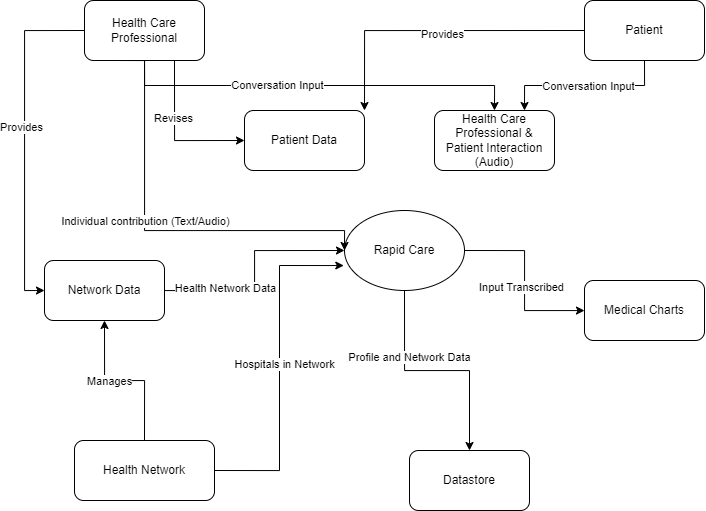
\includegraphics[width=0.8\textwidth]{System_Context.png}
  \caption{This is the System Context diagram for this scenario.}
  % \label{fig:Use-Case Diagram}
\end{figure}
Through this project we aim to develop a solution that will address key niche problems through customizability and add features of critical need that do not already exist in existing solutions. This will allow healthcare networks to centralize the data of their hospitals and increase the staff productivity.\\

\noindent This product has been conceived by the group members based on elicitation. Through interviews and discussion the problem of documentation overhead was found. This is the problem to be solved for the capstone course SFWRENG 4G06.

\begin{itemize}
  \item \textbf{Inputs:}
  \begin{itemize}
    \item Voice dictation from healthcare professionals.
    \item Keyboard typing to amend or edit any documentation.
  \end{itemize}
  \item \textbf{Outputs:}
  \begin{itemize}
    \item Transcription of voice dictation into text.
    \item Segmentation of text into clinical notes.
    \item Saved amendments, creations, and deletions of records.
  \end{itemize}
  \item \textbf{User Responsibilities:}
  \begin{itemize}
    \item Provide voice dictation of conversations.
    \item Amend or delete documentation as needed.
    \item Maintain existing data, and journey tracks.
  \end{itemize}
  \item \textbf{System Responsibilities:}
  \begin{itemize}
    \item Accurate, transcribe voice dictation into text.
    \item Accurate mapping of patient journey in application.
  \end{itemize}

\item{\textbf{Expected Benefits:}}

\begin{itemize}
  \item Reduced documentation overhead time
  \item Increased patient throughput
  \item Improved patient care
  \item Increased doctor and healthcare professional satisfaction
\end{itemize}
\end{itemize}
Much like how copilot is a tool for programmers, the aim is to create a tool for healthcare professionals to help with documentation such that the number of patient processed per day can be increased, and the focus of doctors and nurses can be shifted from documentation to patient care. 


\subsection{User Characteristics} \label{sec_UserCharacteristics}

The intended users of this product are healthcare professionals, specifically those involved in patient documentation, including doctors, nurses, and other clinical administrative staff. Here is the list of potential stakeholders:\\

\begin{itemize}
  \item\textbf{Healthcare Professionals:} These include the hospital staff such as Doctors, nurses etc, who will use the system.
  \item\textbf{Healthcare Network Employees:} These are the people employed in the organization who keeps records of all hospital facilities, their staff members and authenticates the healthcare professionals so that they are able to use the system.
  \item\textbf{Healthcare Institutions:} While society is a major stakeholder in this project, healthcare institutions such as hospitals and clinics are a part of users group within the society. These institutions will be benefitted with improved efficiency in assisting patients. Health, safety, cultural diversity, and other pertinent elements such as waiting times and patient outcomes for the society are taken into account.  
\end{itemize}

The following are the user characteristics associated with the intended users:\\

\begin{itemize}
  \item\textbf{Education Level:} All users are expected to have a minimum of a college diploma and basic reading, writing, and speaking skills. The education level of the intended users will vary based on their role, generally a bachelor's degree or college diploma in nursing, medicine, or other healthcare fields. \\
  \item\textbf{Experience:} All users will be expected to have basic familiarity with EHR systems or similar applications. This experience will depend on their roles ranging from entry-level positions to experienced professionals. \\
  \item\textbf{Technical Expertise:} The users should have basic technical skills to use EHR systems and other healthcare software applications. In addition to this, the users should have familiarity with data entry processes and analytics interpretation. \\
  \item\textbf{Accessibility Considerations:} It is anticipated that some users may have accessibility issues. The user interface should be designed for ease of navigation, incorporating various accessibility featuresm such as providing step-by-step instructions .\\
\end{itemize}

Specific requirements must be specified to accommodate users with varying technical expertise and diverse educational backgrounds. This will ensure the application is usable by all healthcare staff, regardless of their abilities.


\subsection{System Constraints}

The following constraints will guide the system design and implementation:

\begin{itemize} 

  \item \textbf{Compliance with Regulatory Standards:} The system must adhere to healthcare regulations ensuring the confidentiality and security of patient data.

  \item \textbf{User Accessibility:} The system must meet established accessibility standards to ensure usability for all healthcare staff, including those with disabilities.

  \item \textbf{Cost and Time:} The system must be developed within the imposed budget and time restrictions.

\end{itemize}


~\newpage

\section{Specific System Description} \label{sec_SpecificSystemDescription}


\subsection{Problem Description} \label{sec_ProblemDescription}

Ontario is facing an extreme shortage of family doctors, with the number of patients without one jumping by 600,000 to 2.5 million which is a growing number [1]. This situation is only to get worse as predicted by the Ontario Medical Association [2]. As a result, people find themselves going to the ER with coughs and colds and flooding the ER causing massive wait times which ends in patients even resulting in leaving without being seen [3]. A massive part of the wait time is due to the overhead of documentation tasks. Doctors, healthcare professionals, and support staff find themselves spending most of their time on documentation which overall slows the pipeline of patients tremendously.


\subsubsection{Terminology and Definitions} \label{sec_TerminologyDefinitions}

The following is the glossary for this document:

\begin{itemize}
  \item \textbf{System:} The intended solution/product.
  \item \textbf{User:} A person who will use the product.
  \item \textbf{Healthcare Professional:} A doctor, nurse, and other healthcare professional who will be using the product.
  \item \textbf{Patient:} Any person who is receiving medical treatment.
  \item \textbf{Healthcare Network:} An organisation that has group of hospitals or clinics and will use the system.
\end{itemize}


\subsubsection{Physical System Description} \label{sec_phySystDescrip}
N/A


\subsubsection{Goals Statements} \label{sec_Goals}
The goals for this project are as follows:
\begin{table}[H]
    \centering
    \begin{tabular}{p{4cm} p{4cm} p{4cm}}
        \toprule
        \textbf{Goal} & \textbf{Definition} & \textbf{Rationale} \\
        \midrule
        G\refstepcounter{goalnum}\thegoalnum\label{G_VoiceToDocumentation}: Use voice to fill in medical documentation (charts, files, etc.) & The app will record conversations and automatically turn them into medical notes and charts. & This will save doctors time by automating paperwork, letting them focus more on patients. \\
        \midrule
        G\refstepcounter{goalnum}\thegoalnum \label{G_reduceOverhead}: Reduce documentation overhead time.  & Through tracking the whole patient journey in the app, we look to reduce the overhead of triaging, clinical documentation, and other registrations.  & This helps hospital healthcare professionals focus on care and lowers the time taken through registration for hospital staff. \\ 
        \midrule
        G\refstepcounter{goalnum}\thegoalnum \label{G_integrateEnv}: Integrates with the existing hospital environment. & We want the solution to be portable such that it can be implemented in existing hospital and clinic ecosystems.  & Portability will ensure that hospitals and clinics won't have to upgrade their existing hardware to use the application. \\
        \midrule 
        G\refstepcounter{goalnum}\thegoalnum \label{G_hNetworkProfiles}: Allow health networks profiles with in service. & Need the ability for health networks to add, update, and delete network profile details. & This will ensure that the list of hospitals and staff in the network is up to date with appropriate permissions. \\
        \midrule 
        G\refstepcounter{goalnum}\thegoalnum \label{G_hProfessionalProfiles}: Allow health care professional profiles with in service. & Need the ability for health networks to add, update, and delete staff profile details. & This will ensure that the list of staff will be able to use the tool to dictate patient conversations or add other notes. Additionally, making sure they have access to patient journey. \\
        \midrule 
        G\refstepcounter{goalnum}\thegoalnum \label{G_medicineSuggestions}: Automated medicine suggestions. & Based on diagnosis and patient data provide medicine suggestions. & This will help doctors fill out their charts faster. \\ % Row 1
        \midrule 
        G\refstepcounter{goalnum}\thegoalnum \label{G_diagnosisSuggestions}: Automated diagnosis suggestions.  & Use AI to suggest possible diagnoses based on what the doctor and patient discuss.  & This will help doctors make faster, more accurate diagnoses, especially in tricky cases.\\ 
    \end{tabular}
\end{table}

\subsubsection{Stretch Goals} \label{sec_StretchGoals}
The stretch goals for this project are as follows:
\begin{table}[H]
    \centering
    \begin{tabular}{p{4cm} p{4cm} p{4cm}}
        \toprule
        \textbf{Goal} & \textbf{Definition} & \textbf{Rationale} \\
        % \midrule
        % STG\refstepcounter{stretchgoalnum}\thestretchgoalnum \label{STG_medicineSuggestions}: Automated medicine suggestions. & Based on diagnosis and patient data provide medicine suggestions. & This will help doctors fill out their charts faster. \\ % Row 1
        \midrule
        % STG\refstepcounter{stretchgoalnum}\thestretchgoalnum \label{STG_diagnosisSuggestions}: Automated diagnosis suggestions.  & Use AI to suggest possible diagnoses based on what the doctor and patient discuss.  & This will help doctors make faster, more accurate diagnoses, especially in tricky cases.\\ 
        \midrule
        STG\refstepcounter{stretchgoalnum}\thestretchgoalnum \label{STG_triage}: Increase efficiency for triage.  & Create functionality to prioritize patients based on the severity of their condition. & This ensures the most critical patients get treated first, improving care in emergencies. \\
        \bottomrule
    \end{tabular}
\end{table}


\subsection{Solution Characteristics Specification} \label{sec_SolutionCharacteristicsSpecification}

This section outlines the core functionalities and characteristics of the proposed system:

\begin{itemize}
  \item \textbf{Patient Documentation:} The system should facilitate efficient and streamlined patient documentation throughout the EHR documentation process. This includes storing patient data, clinical notes, treatment plans, and patient history in a secure manner.
  
  \item \textbf{Voice Transcription:} The system should be able to record conversations between healthcare professionals and patients which will be transcribed to fill out charts and patient profiles efficiently.
  
  \item \textbf{Real-time Data Access:} The users must have real-time access to patient data and documentation enabling them to make informed decisions quickly and efficiently.
  
  \item \textbf{Automated Medicine Suggestions:} The system should be able to provide automated medicine suggestions based on the transcribed data which will help users to fill out the charts faster and make informed treatment decisions.
  
  \item \textbf{Automated Diagnosis Suggestions:} The system should be able to suggest possible diagnoses based on transcribed data which will help users to make faster and more accurate diagnoses.
  
  \item \textbf{User Authentication:} The system must provide secure user authentication methods to ensure that only authorized personnel can access sensitive patient information.
  
\end{itemize}

\subsubsection{Types} \label{sec_Types}
N/A

\subsubsection{Scope Decisions} \label{sec_ScopeDecisions}
N/A

\subsubsection{Modelling Decisions} \label{sec_ModellingDecisions}
N/A


\subsubsection{Assumptions} \label{sec_assumpt}

\begin{itemize}
  \item[A\refstepcounter{assumpnum}\theassumpnum \label{A_reliableInternet}:] \textbf{Reliable Internet Connection:} We assume that the user has a reliable internet connection throughout their operational hours.
  \item[A\refstepcounter{assumpnum}\theassumpnum \label{A_sufficientHardware}:] \textbf{Sufficient Hardware Accessories:} We are assuming that the user has the required hardware devices such as monitors, iPads etc. to access the system.
  \item[A\refstepcounter{assumpnum}\theassumpnum \label{A_patientConsent}:] \textbf{Patient's Consent:} We also assume that medical staff will obtain patients' consent when required.  
\end{itemize}


\subsubsection{Theoretical Models}\label{sec_theoretical}
N/A

\subsubsection{General Definitions} \label{sec_GeneralDefinitions}
N/A

\subsubsection{Data Definitions}\label{sec_DataDefinitions} 
N/A

\subsubsection{Data Types}\label{sec_DataTypes}
N/A

\subsubsection{Instance Models} \label{sec_InstanceModels} 
N/A

\subsubsection{Input Data Constraints} \label{sec_InputDataConstraints}
N/A


\subsubsection{Properties of a Correct Solution} \label{sec_CorrectSolution}

Since this is a software application, the properties of correctness can be described through its core use-case scenarios for the system:

\begin{itemize}
  \item\textbf{UC1 Login:}
  \begin{itemize}
    \item The user accesses the system using an internet browser.
    \item The user enters valid credentials on the log in page.
    \item The user selects the login button.
    \item The user lands on the default dashboard.
  \end{itemize}
  \item\textbf{UC2 Recording Clinical Notes:}
  \begin{itemize}
    \item The user accesses patient's record.
    \item The user initiates dictation.
    \item The user dictates the notes and hit the stop button.
    \item The user reviews the transcribed text.
    \item The user selects the submit button.
  \end{itemize}
  \item\textbf{UC3 Diagnostic Suggestions:}
  \begin{itemize}
    \item The user submits the transcribed text.
    \item The user reviews the potential diagnostic suggestions.
    \item The user accepts or rejects suggestions.
  \end{itemize}
  \item\textbf{UC4 Create Patient Profile:}
  \begin{itemize}
    \item The user log into the system.
    \item The user selects the 'create a new record' button.
    \item The user provide input for the required fields.    
    \item The user selects the submit button.
  \end{itemize}
\end{itemize}

\begin{figure}[H]
  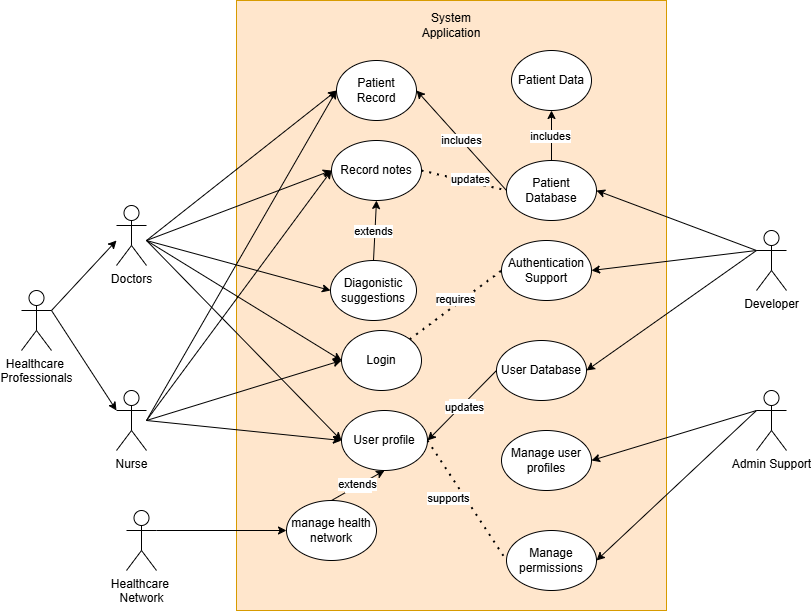
\includegraphics[width=0.8\textwidth]{use-case.drawio.png}
  \caption{This is the use-case diagram for this scenario.}
  \label{fig:Use-Case Diagram}
\end{figure}

\textbf{Main Usage Scenario: Documenting a Patient Consultation}

\begin{itemize}
  \item\textbf{Use Case:} UC2, UC3
  \item\textbf{Primary Actor:} Healthcare professional (such as a medical doctor or a nurse)
  \item\textbf{Precondition:} The user has been successfully authenticated, logged into the system and has patient's profile is created. The basic information such as name, contact information, and history is prefilled.
  \item\textbf{Trigger:} The user will initiate dictation.
  \item\textbf{Main Success Scenario:}
  \begin{itemize}
    \item The user will initiate dictation.
    \item The system will convert audio to text in real-time.
    \item The user will press stop button.
    \item The user reviews the transcribed notes. 
    \item The system has accurately transcribed the audio to text without any inaccuracies.
    \item The user selects the submit button after review. 
  \end{itemize}
  \item\textbf{Secondary Success Scenario:}
  \begin{itemize}
    \item The system has produced some inaccuracies in the transcribed text.
    \begin{itemize}
      \item The user selects the edit button.
      \item The system prompts user to edit the text.
      \item The user manually edits the transcribed text.
    \end{itemize} 
  \end{itemize}
  \item\textbf{Success Postcondition:}
  \begin{itemize}
    \item The notes are successfully saved in patient database and changes are reflected in the user interface.
  \end{itemize}
\end{itemize}

\subsubsection{Risks and Mitigation}

Following are the anticipated risks in this project. If these risks can be addressed or have a clearer roadmap that will make us more confident in the project. 

\begin{itemize}
  \item \textbf{Speech Input:} A hospital or a clinic can be a loud place, in the event audio input is taken we need to ensure that it is clean and clear. This would mean essentially blocking outside noise. 
  \item \textbf{Pre-Trained Models:} To manipulate and use both inputs above we need to create a model to be accurate and provide accuracy when filling in charts. 
  \item \textbf{User Acceptance:} This will require further elicitation from outside supervisors. We need to gather data on what critical needs of healthcare professionals such that critical features are present.
  \item \textbf{Technical Delay:} Integration with EHR systems might cause some delays if there's any technical issue or if the software faces compatibility issues. This will require sample testing to make sure that the system is compatible in the early stage of the development process.
  \item \textbf{Professional Verification:} Misinterpretation of some words might lead to inaccurate records and wrong diagnosis. Therefore, it's important for the healthcare professionals to verify the final version of the document and manually delete anything that was falsely recorded. 
\end{itemize}

~\newpage

\section{Requirements} \label{sec_Requirements}


\subsection{Functional Requirements} \label{sec_FunctionalRequirements}


\noindent \begin{itemize}

\item [FR\refstepcounter{reqnum}\thereqnum \label{FR_addHealthNetwork}:] 

\textbf{Requirement:} The system should allow a healthcare network to be onboarded to the system.

\textbf{Rationale:} Rapid care is an organizational tool, where networks can register their various hospitals, and in turn add the corresponding health care professionals. When the networks want to register, the app needs to be able to add the network to the database along with the relevant staff profiles etc.

\textbf{Fit Criterion:} The network data and profiles are fully added to the database. This could be verified by returning the valid entries from the patient database.

\textbf{Dependencies:} N/A

\textbf{Monitored and Controlled Variables:} N/A

\textbf{Performance Requirements:} 
\begin{itemize}
  \item The system should update the entries with the latency of 1 second.
  \item After user input is taken the system only adds valid entries to the database and prevents any data leaks.
\end{itemize}

\textbf{Hardware Requirements:} 
\begin{itemize}
  \item Workstations and other peripherals to access the system.
\end{itemize}

\textbf{Software Requirements:} 
\begin{itemize}
  \item Database management system to store health network data.
  \item Internet browser to access the application.
\end{itemize}

\textbf{Normal Behavior:} 
\begin{itemize}
  \item All input data is validated as being entered into the system.
  \item Once all required fields are completed the user selects the submits the information and the network is added successfully to the system.
  \item The process should have a low turnover time such that health networks will not have to spend a long time waiting to use the system.
\end{itemize}

\textbf{Undesired Event Handling:} 
\begin{itemize}
  \item The user may enter invalid input data. The system should display appropriate error messages. 
  \item The system should have constraints to restrict the user from submitting, unless all required fields are completed and have valid input data. 
  \item When the database is overloaded with requests, appropriate error messages should be delayed. 
  \item The updates will be queued to prevent this in the future, data resources will be scaled just so that the calls are faster.
\end{itemize}


\item[FR\refstepcounter{reqnum}\thereqnum \label{FR_removeHealthNetwork}:]  

\textbf{Requirement:} The system should allow health network to remove itself from the system.

\textbf{Rationale:} 
When health networks close and want to pivot to another documentation tool their data and profiles must be deleted. Therefore, there is a requirement for functionality that allows organizations to deregister and have their data deleted.

\textbf{Fit Criterion:} 
The network data and profiles are fully deleted from the database. This could be verified by returning the valid entries from the patient database.

\textbf{Dependencies:} FR\ref{FR_addHealthNetwork} 

\textbf{Monitored and Controlled Variables:} N/A

\textbf{Performance Requirements:} 
\begin{itemize}
  \item The removal process must be easy to complete with a latency of 1 second. 
  \item The system should be able to identify the correct record to delete. 
  \item The system should delete the correct record without affecting the rest of the database. 
\end{itemize}

\textbf{Hardware Requirements:} 
\begin{itemize}
  \item Workstations and other peripherals to access the system.
\end{itemize}

\textbf{Software Requirements:}
\begin{itemize}
  \item Access to health network database.
  \item Internet browser to access the application.
\end{itemize}

\textbf{Normal Behavior:}
\begin{itemize}
  \item Network is successfully removed from database with low turnover time such that health networks will not have to spend a long time waiting for their data to be deleted.
\end{itemize}

\textbf{Undesired Event Handling:}
\begin{itemize}
  \item If the system fails to delete the health network due to a system error, the system should display an appropriate error message. 
  \item When the database is overloaded with requests, the operation to delete all the hospital data will be queued as the next action in line.
\end{itemize}


\item[FR\refstepcounter{reqnum}\thereqnum \label{FR_UpdateHealthNetwork}:]

\textbf{Requirement:} The healthcare network should be able to update its organizational and hospital information.

\textbf{Rationale:} The healthcare network will update its own organizational changes. This will include creating and maintaining the staff present as well as the hospitals in the network.

\textbf{Fit Criterion:} The healthcare network data will be up to date with its current state (i.e. number of hospitals, staff etc.), the data's recency will depend on the networks need. 

\textbf{Dependencies:} FR\ref{FR_addHealthNetwork}

\textbf{Monitored and Controlled Variables:} N/A

\textbf{Performance Requirements:} 
\begin{itemize}
  \item The updating process of healthcare networks should be quick and easy so that healthcare professionals remain up to date with the facility information, operational data, healthcare professional data, and patient data.
\end{itemize}

\textbf{Hardware Requirements:} 
\begin{itemize}
  \item Workstations and other peripherals to access the system.
\end{itemize}

\textbf{Software Requirements:} 
\begin{itemize}
  \item Internet browser to access the application.
\end{itemize}

\textbf{Normal Behavior:}
\begin{itemize}
  \item Network is updated in the database without any leaks or latency.
  \item Normal behavior will be seen as updated reflected on the front-end and backend of the system.
\end{itemize} 

\textbf{Undesired Event Handling:} 
\begin{itemize}
  \item When the health network data is being updated and the database is overloaded with requests, then updates will be queued.
\end{itemize}

\item[FR\refstepcounter{reqnum}\thereqnum \label{FR_AddHealthProfessional}:]

\textbf{Requirement:} The system should allow healthcare network administrators to add healthcare professionals to the system.

\textbf{Rationale:} When new healthcare professionals join the healthcare network, their information is to be added to the system for authentication purposes. This will include adding a list of hospital staff members to the network.

\textbf{Fit Criterion:} The healthcare professional's data will be up to date in the system so that they can get authenticated without any delay. 

\textbf{Dependencies:} N/A 

\textbf{Monitored and Controlled Variables:} N/A

\textbf{Performance Requirements:} 
\begin{itemize}
  \item The addition process should be quick and easy to ensure that all professionals can access the database without any interruptions.
\end{itemize}

\textbf{Hardware Requirements:} 
\begin{itemize}
  \item Workstations and other peripherals to access the system.
\end{itemize}

\textbf{Software Requirements:} 
\begin{itemize}
  \item Internet browser to access the database.
\end{itemize}

\textbf{Normal Behavior:}
\begin{itemize}
  \item Data is added to the database without any leaks or latency. Normal behavior will be seen as updated are reflected in database and UI of the system.
\end{itemize} 

\textbf{Undesired Event Handling:}
\begin{itemize}
  \item When the healthcare professional's data is being added and the database is overloaded with requests, then updates will be queued.
\end{itemize} 

\item[FR\refstepcounter{reqnum}\thereqnum \label{FR_RemoveHealthProfessionals}:] 

\textbf{Requirement:} The system should allow healthcare network administrators to remove healthcare professionals from the system. 

\textbf{Rationale:} Sometimes a healthcare professional decides to change the area of service or leaves the organization and retires. Therefore, there is a need for functionality that allows to remove them from the system.

\textbf{Fit Criterion:} The healthcare professional is successfully removed from the system, this will be verified by the fact that they are not present in the databases. 

\textbf{Dependencies:} FR\ref{FR_AddHealthProfessional}

\textbf{Monitored and Controlled Variables:} N/A

\textbf{Performance Requirements:}
\begin{itemize}
  \item The deleting process must be easy to complete with a low turnover time such that health networks will not have to spend a long time waiting for their data to be deleted.
\end{itemize} 

\textbf{Hardware Requirements:}
\begin{itemize}
  \item Workstations and other peripherals to access the system.
\end{itemize} 

\textbf{Software Requirements:}
\begin{itemize}
  \item Internet browser to access the database.
\end{itemize} 

\textbf{Normal Behavior:}
\begin{itemize}
  \item Data is removed to the database without any leaks or latency. Normal behavior will be seen as updated are reflected on the frontend and backend of the system.
\end{itemize} 

\textbf{Undesired Event Handling:}
\begin{itemize}
  \item When the healthcare professional's data is being removed and the database is overloaded with requests, then updates will be queued.
\end{itemize} 

\item[FR\refstepcounter{reqnum}\thereqnum \label{FR_UpdateHealthProfessionals}:]

\textbf{Requirement:} The system should allow healthcare network administrators to update healthcare professional's data in the system.

\textbf{Rationale:} Sometimes healthcare professionals receive promotions or other changes in their roles which require updating the information in their profiles. Therefore, it is essential for functionality that allows to edit the data in case there are inaccuracies.  

\textbf{Fit Criterion:} The healthcare professional's data will be up to date in its current state (i.e. role of each healthcare professional and the organization they work in etc). 

\textbf{Dependencies:} FR\ref{FR_AddHealthProfessional}

\textbf{Monitored and Controlled Variables:} N/A

\textbf{Performance Requirements:} 
\begin{itemize}
  \item The changes should be reflected in real time on the UI.
  \item The changes should be stored successfully in the database.
\end{itemize} 

\textbf{Hardware Requirements:}
\begin{itemize}
  \item Workstations and other peripherals to access the system.
\end{itemize} 

\textbf{Software Requirements:}
\begin{itemize}
  \item Internet browser to access the database.
\end{itemize} 

\textbf{Normal Behavior:}
\begin{itemize}
  \item Data is updated in the database without any leaks or latency. Normal behavior will be seen as updated are reflected on the front-end and backend of the system.
\end{itemize} 

\textbf{Undesired Event Handling:}
\begin{itemize}
  \item When the healthcare professional's data is being updated and the database is overloaded with requests, then updates will be queued.
\end{itemize} 

\item[FR\refstepcounter{reqnum}\thereqnum \label{FR_login}:]

\textbf{Requirement:} The system should allow the authorized user to successfully log in to the system.

\textbf{Rationale:} Doctors and other medical professionals should be able to log into the system to create patients, update, and delete patient records and access their medical records. The system should also authenticate the user to avoid unauthorized access to the data.

\textbf{Fit Criterion:} The system only authenticates the authorized users to log into the system and has 100\% accuracy. 

\textbf{Dependencies:} FR\ref{FR_AddHealthProfessional}, FR\ref{NFR_Security}

\textbf{Monitored and Controlled Variables:} number of failed login attempts

\textbf{Performance Requirements:} 
\begin{itemize}
  \item The system successfully redirects users to correct system state based on authentication.
\end{itemize}

\textbf{Hardware Requirements:} 
\begin{itemize}
  \item Workstations and other peripherals to access the system.
\end{itemize}

\textbf{Software Requirements:} 
\begin{itemize}
  \item Authentication protocols and encryption for security. 
  \item Internet browser to access the system.
\end{itemize}

\textbf{Normal Behavior:} 
\begin{itemize}
  \item The user is able to successfully login upon providing valid credentials and is redirected to the appropriate dashboard based on their role.
\end{itemize}

\textbf{Undesired Event Handling:}
\begin{itemize}
  \item If a user provides invalid credentials, the system will display an error message and redirect the user to sign in page.
  \item After three failed login attempts, the user account will be locked, and the user will have to contact the support team to regain access.
\end{itemize}
 

\item[FR\refstepcounter{reqnum}\thereqnum \label{FR_createRecord}:]

\textbf{Requirement:} The user should be able to create a new patient record. 

\textbf{Rationale:} The patient data and medical history must be stored in a secure manner. Therefore, medical staff should be able to create a new patient record to store all the relevant information. 

\textbf{Fit Criterion:} The record is created and added to the patient database. This could be verified by returning the valid entries from the patient database.

\textbf{Dependencies:} FR\ref{FR_login}

\textbf{Monitored and Controlled Variables:} field validation

\textbf{Performance Requirements:} 
\begin{itemize}
  \item The system should update the patient database with the latency of 1 second. 
  \item The system only adds valid entries to the database.
  \item The system prevents any data leaks.
\end{itemize}

\textbf{Hardware Requirements:} 
\begin{itemize}
  \item Workstations and other peripherals to access the system.
\end{itemize}

\textbf{Software Requirements:} 
\begin{itemize}
  \item Database management system to store patient information.
  \item Internet browser to access the system.
\end{itemize}

\textbf{Normal Behavior:} 
\begin{itemize}
  \item All input data is validated as it is entered using field level validation. 
  \item Once all required fields are completed the user selects the submit button, a new patient record is successfully created and stored.
\end{itemize}

\textbf{Undesired Event Handling:} 
\begin{itemize}
  \item The user may enter invalid input data. The system should display appropriate error messages. 
  \item The system should have constraints to restrict the user from submitting, unless all required fields are completed and have valid input data. 
  \item If the system fails to save the record due to a system error, the system should display an appropriate error message. 
\end{itemize}


\item[FR\refstepcounter{reqnum}\thereqnum \label{FR_deleteRecord}:]

\textbf{Requirement:} The user should be able to delete an existing patient record from the system.

\textbf{Rationale:} There can be instances where medical professionals need to delete a certain patient record, for example inaccurate entries, duplicate records etc. Therefore, the system should allow authorized users to remove patient records.

\textbf{Fit Criterion:} The record is successfully removed from the patient database. This could be verified by returning the valid entries from the patient database.

\textbf{Dependencies:} FR\ref{FR_login}, FR\ref{FR_createRecord}

\textbf{Monitored and Controlled Variables:} N/A

\textbf{Performance Requirements:} 
\begin{itemize}
  \item The deletion process must be easy to complete with a latency of 1 second. 
  \item The system should be able to identify the correct record to delete. 
  \item The system should delete the correct record without affecting the rest of the database. 
\end{itemize}

\textbf{Hardware Requirements:} 
\begin{itemize}
  \item Workstations and other peripherals to access the system.
\end{itemize}

\textbf{Software Requirements:} 
\begin{itemize}
  \item Access to patient record database.
  \item Role based access control system to manage user permissions.
  \item Internet browser to access the system.
\end{itemize}

\textbf{Normal Behavior:} 
\begin{itemize}
  \item The user selects the delete button and confirms the deletion. The patient record is successfully removed from the database and no longer appears on the system.
\end{itemize}

\textbf{Undesired Event Handling:} 
\begin{itemize}
  \item If the user does not have permission to delete the record, the system should show an appropriate error message.
  \item If the system fails to delete the record due to a system error, the system should display an appropriate error message. 
\end{itemize}



\item[FR\refstepcounter{reqnum}\thereqnum \label{FR_updateRecordtyping}:]

\textbf{Requirement:} : The system should allow the user to update the patient records manually by typing.

\textbf{Rationale:} Medical professionals frequently need to update patient information, such as changes in diagnosis, medication, or medical history. The healthcare professional may want to add some information manually. Moreover, if healthcare professionals use the dictation tool, they still should be allowed to edit the auto filled transcribed data in case there are inaccuracies.

\textbf{Fit Criterion:} The system should update the current state and patient database with the input information.

\textbf{Dependencies:} FR\ref{FR_login}, FR\ref{FR_createRecord}

\textbf{Monitored and Controlled Variables:} N/A

\textbf{Performance Requirements:} 
\begin{itemize}
  \item The changes should be reflected in real time on the user interface.
  \item The changes should be stored successfully in the database.
\end{itemize}

\textbf{Hardware Requirements:} 
\begin{itemize}
  \item Workstations and other peripherals to access the system.
\end{itemize}

\textbf{Software Requirements:} 
\begin{itemize}
  \item Access to patient record database.
  \item Internet browser to access the system. 
\end{itemize}

\textbf{Normal Behavior:} 
\begin{itemize}
  \item The user edits the selected field and enters new information. 
  \item The system successfully updates the changes in database and reflect changes on the user interface. 
\end{itemize}

\textbf{Undesired Event Handling:}
\begin{itemize}
  \item If an unauthorized user tries to update a record, the system displays appropriate error messages. 
  \item If the system fails to update the record due to a system error, the system should display an appropriate error message. 
\end{itemize}

\item[FR\refstepcounter{reqnum}\thereqnum \label{FR_DictationRecording}:]

\textbf{Requirement:} The system should allow healthcare workers to update patient records using dictation. 
    
\textbf{Rationale:} This will reduce the workload on the healthcare workers, while also efficiently reducing the time spent on documentation. 
    
\textbf{Fit Criterion:} The system should use voice dictation to document medical reports with a minimum of 90\% accuracy. 
    
\textbf{Dependencies:} FR\ref{FR_login}, FR\ref{FR_createRecord} 
    
\textbf{Monitored Variables:} Accuracy
    
\textbf{Performance:} 
  \begin{itemize}
      \item System should transcribe speech in real time and segment it into the right fields onto the record with a minimum of 90\% accuracy.
  \end{itemize}
    
\textbf{Hardware Requirements:}
  \begin{itemize}
      \item Workstations to access the system and a microphone which can record the voice in the system. 
  \end{itemize}
    
\textbf{Software Requirements:}
  \begin{itemize}
      \item An audio transcription service to transcribe audio to text 
      \item Access to patient record database. 
      \item Internet browser to access the system.  
  \end{itemize}
    
\textbf{Normal Use:} 
\begin{itemize}
  \item The system records the provider's voice and updates the patient file with the transcribed text.
\end{itemize}
    
\textbf{Undesired Event Handling:} 
\begin{itemize}
  \item If the recording or transcription fails, the system should notify the user and offer manual review.
\end{itemize}


\item[FR\refstepcounter{reqnum}\thereqnum \label{FR_DiagnosticSuggestions}:]

\textbf{Requirement:} The system should analyze transcribed text and provide diagnostic suggestions based on the input.
    
\textbf{Rationale:} This alerts the healthcare professionals about the possible diagnostics and helps them to diagnose the patients quicker based on suggested options.
    
\textbf{Fit Criterion:} The system must suggest diagnoses within 5 seconds after transcript is provided, with 85\% accuracy based on known patient's medical record.
    
\textbf{Dependencies:} FR\ref{FR_DictationRecording}
    
\textbf{Monitored Variables:} Suggested diagnostic accuracy, time to generate suggestions 
  
\textbf{Performance:}
  \begin{itemize}
    \item Suggestions must be provided within 5 seconds of transcript completion. 
    \item Suggestions should match known diagnoses with 85\% accuracy. 
  \end{itemize}
    
\textbf{Hardware Requirements:}
  \begin{itemize}
    \item Workstations and other peripherals to access the system. 
  \end{itemize}
    
\textbf{Software Requirements:}
  \begin{itemize}
    \item Access to patient record database. 
    \item Internet browser to access the system.  
    \item Service engine that generates diagnostic suggestions. 
  \end{itemize}
    
\textbf{Normal Use:} 
  \begin{itemize}
    \item The system analyzes the transcribed conversation and suggests possible diagnoses based on a patient's medical record. 
  \end{itemize}
    
\textbf{Undesired Event Handling:} 
  \begin{itemize}
    \item If the system can't suggest a diagnosis, it should notify the user and offer a manual search option. 
  \end{itemize}


\item[FR\refstepcounter{reqnum}\thereqnum \label{FR_medicalSuggestions}:] 

\textbf{Requirement:} The system should provide a list of frequently used medicines based on accepted diagnosis.

\textbf{Rationale:} As the patients' medical records and data is being added into the charts, having a model that can provide a preliminary set of diagnosis such that documentation time can be saved. This supplementary tool will provide auto-completion analogous to what auto-completion tools programmers use.

\textbf{Fit Criterion:} Auto-completion suggestions regarding diagnoses and medicine are applicable 85+\% of the time. The model will be measured through cross validation techniques.
 
\textbf{Dependencies:} FR\ref{FR_DictationRecording}, FR\ref{FR_DiagnosticSuggestions}

\textbf{Monitored and Controlled Variables:} accuracy

\textbf{Performance Requirements:}
\begin{itemize}
  \item The autocompletion is accurate, such that it is correct 85+\% of the time. 
\end{itemize}

\textbf{Hardware Requirements:} 
Workstations and other peripherals to access the system.

\textbf{Software Requirements:}
\begin{itemize}
  \item Access to patient record database.
  \item Internet browser to access the system. 
\end{itemize}

\textbf{Normal Behavior:}
\begin{itemize}
  \item A list of medicine suggestion is provided almost instantly analogous to an auto-complete feature based on the selected diagnosis.
\end{itemize}

\textbf{Undesired Event Handling:}
\begin{itemize}
  \item In case no medicine suggestions are provided the doctor can manually add a prescription.
\end{itemize}

\item[FR\refstepcounter{reqnum}\thereqnum \label{FR_transferPatient}:] 
\textbf{Requirement:} The system should be able to transfer patient documentation to another provider. 

\textbf{Rationale:} If the patient goes to a hospital in another health network, perhaps the medical history is to be shared. This functionality will allow the request and transfer of files.

\textbf{Fit Criterion:} Transfer over the files in a short time, the transfer protocol is secure, and data is not leaked.

\textbf{Dependencies:} FR\ref{FR_createRecord}

\textbf{Monitored and Controlled Variables:} N/A

\textbf{Performance Requirements:}
\begin{itemize}
  \item The system should transfer data with low latency.
\end{itemize}

\textbf{Hardware Requirements:} 
\begin{itemize}
  \item Workstations and other peripherals to access the system.
\end{itemize}

\textbf{Software Requirements:}
Access to patient record database.
\begin{itemize}
  \item Internet browser to access the system. 
\end{itemize}

\textbf{Normal Behavior:}
\begin{enumerate}
  \item A patient file is requested
  \item The request is approved then the files are transferred.
\end{enumerate}
-
\textbf{Undesired Event Handling:}
\begin{enumerate}
  \item A patient file is requested 
  \item The request for the file is denied. 
  \item A detailed request is submitted for approval to provide further information that may have been missing.
\end{enumerate}
\end{itemize}
\subsection{Non-functional Requirements} \label{sec_NonFunctionalRequirements}

\noindent \begin{itemize}

\item[NFR\refstepcounter{nfrnum}\thenfrnum \label{NFR_LookAndFeel}:] \textbf{Aesthetic and Design}

    \textbf{Requirement:} The UI should have a clean design that prioritizes simplicity and ease of navigation.

    \textbf{Rationale:} A clean user interface allows users to navigate through the application with ease. We want to reduce excess noise and make the UI as simple as possible.

    \textbf{Fit Criterion:} UI prototypes will be tested with healthcare workers to confirm that they find the interface easy to use and navigate, with primary functions accessible within two clicks from the main screen.

    \textbf{Dependencies:} N/A

    \textbf{Undesired Event Handling:} If the surveys shows less than 80\% satisfaction, UI will be revised.


\item[NFR\refstepcounter{nfrnum}\thenfrnum \label{NFR_Usability}:] \textbf{Usability}

    \textbf{Requirement:} The UI must be highly intuitive, ensuring high discoverability of all system functions.

    \textbf{Rationale:} If the UI is user-friendly, it tends to reduce the learning time and allows health care workers to focus on patients. Additionally, we want the functionality to be easy to discover such that the user does not have to spend time searching for a feature.
  
    \textbf{Fit Criterion:} Usability tests will demonstrate that 90\% of healthcare workers can effectively use the system after 30 minutes of training.

    \textbf{Dependencies:} NFR\ref{NFR_LookAndFeel}

    \textbf{Undesired Event Handling:} If user satisfaction is low the system should have clear documentation and training materials to help the user learn the system.

\item[NFR\refstepcounter{nfrnum}\thenfrnum \label{NFR_Performance}:] \textbf{Performance}

    \textbf{Requirement:} The system shall provide responsive voice-to-text conversion and maintain high processing throughput during peak operational loads.

    \textbf{Rationale:} Reduces the documentation time to reduce workload and allow healthcare workers to focus on patients. Real time transcription will allow for lower friction when documenting.
    
    \textbf{Fit Criterion:} The system will consistently generate completed transcription live or off a recording within 30 seconds. Additionally, the accuracy will be greater than 85\%.

    \textbf{Dependencies:} NFR\ref{NFR_Operational}, FR\ref{FR_DictationRecording}

    \textbf{Undesired Event Handling:} In case of transcription delay or failure, feedback regarding the transcription will be provided to the user.

\item[NFR\refstepcounter{nfrnum}\thenfrnum \label{NFR_Operational}:] \textbf{Operational Requirement}

    \textbf{Requirement:} The system must maintain a 99.9\% uptime during operational hours and implement real-time data duplicationm across multiple servers to mitigate data loss.

    \textbf{Rationale:} Reliable uptime ensures consistent system for healthcare workers, specially in time-sensitive atmospheres like hospitals.

    \textbf{Fit Criterion:} System logs will validate that the 99.9\% uptime is maintained over a 30-day period. Different servers should engage in the backup process, with real-time data replication ensuring minimal data loss. 

    \textbf{Dependencies:} N/A
    
    \textbf{Undesired Event Handling:} Data should be duplicated across different servers to ensure consistency. In case of downtime, it should be stored in temporary data containers before starting the syncing process.

\item[NFR\refstepcounter{nfrnum}\thenfrnum \label{NFR_Maintainability}:] \textbf{Maintainability Requirement}

    \textbf{Requirement:} The system shall undergo regular updates for bug fixes and feature enhancements, ensuring minimal disruption.

    \textbf{Rationale:} Easily maintained system allows for consistent service, and allows for extension of features. Also, regular maintenance supports long-term reliability and adaptability of the system.

    \textbf{Fit Criterion:} Update logs will show periodic patches and updates at least once per quarter, with minimal downtime.

    \textbf{Dependencies:} N/A

    \textbf{Undesired Event Handling:} If an update fails, the system will automatically revert to the last stable version.

\item[NFR\refstepcounter{nfrnum}\thenfrnum \label{NFR_Security}:] \textbf{Security Requirement}

    \textbf{Requirement:} The system should have all patient data encrypted, and in compliance with Personal Information Protection and Electronic Documents Act (PIPEDA) standards.

    \textbf{Rationale:} A secure and confidential system ensures the user to be confident in using the application while protecting sensitive patient data.

    \textbf{Fit Criterion:} Security audits will confirm full compliance with PIPEDA, encryption and data protection standards.  

    \textbf{Dependencies:} N/A

    \textbf{Undesired Event Handling:} If a security breach is detected, all users will be logged out, access will be locked, and administrators alerted.

\item[NFR\refstepcounter{nfrnum}\thenfrnum \label{NFR_Cultural}:] \textbf{Cultural Requirement}

    \textbf{Requirement:} The system should allow customization of language settings to accommodate all healthcare workers.

    \textbf{Rationale:} A customized UI allows the user to feel comfortable and confident when using the application.

    \textbf{Fit Criterion:} Tests will show that healthcare workers can navigate through the application and switch languages based on their preference without impacting the functionality of the application.

    \textbf{Dependencies:} N/A

    \textbf{Undesired Event Handling:} If a language bundle fails to load, the system will revert to the default language and notify the user.

\item[NFR\refstepcounter{nfrnum}\thenfrnum \label{NFR_Legal}:] \textbf{Legal Requirement}

    \textbf{Requirement:} The system should comply with all healthcare data protection regulations. 

    \textbf{Rationale:} Legal compliance is necessary to ensure patient data protection and avoid potential legal penalties.  

    \textbf{Fit Criterion:} Legal audits will confirm full compliance with PIPEDA and any other relevant data protection laws.  

    \textbf{Dependencies:} N/A

    \textbf{Undesired Event Handling:} If the system fails to comply with regulations, it will be updated within 24 hours to meet compliance.

\item[NFR\refstepcounter{nfrnum}\thenfrnum \label{NFR_Scalability}:] \textbf{Scalability Requirement}

    \textbf{Requirement:} The system must scale horizontally to handle an increase in concurrent users and data processing load without hindering performance.

    \textbf{Rationale:} Scalability ensures that the system can support growth and increased usage, maintaining performance across multiple healthcare facilities.  

    \textbf{Fit Criterion:}  Stress tests will confirm that the system can support a large number of concurrent users and processes data without a drop in performance.  

    \textbf{Dependencies:} N/A

    \textbf{Undesired Event Handling:} If the system encounters performance bottlenecks, horizontal scaling solutions will be deployed to distribute the load effectively.

\end{itemize}

\subsection{Rationale}

Already completed.

\section{Phase-In Plan}

All requirements with High priority must be implemented prior to the Revision 0 demonstration as they represent the core functionality of our system.\\
FR\ref{FR_AddHealthProfessional}\\
FR\ref{FR_login}\\
FR\ref{FR_createRecord}\\
FR\ref{FR_deleteRecord}\\
FR\ref{FR_updateRecordtyping}\\ 
FR\ref{FR_DictationRecording}\\

All requirements with Medium priority will be implemented before the Revision 1 demonstration.\\
FR\ref{FR_addHealthNetwork}\\
FR\ref{FR_DiagnosticSuggestions}\\
FR\ref{FR_medicalSuggestions}\\

All requirements with Low priority will be added after all High and Medium requirements are implemented, time permitting.\\
FR\ref{FR_removeHealthNetwork}\\
FR\ref{FR_UpdateHealthNetwork}\\
FR\ref{FR_RemoveHealthProfessionals}\\
FR\ref{FR_UpdateHealthProfessionals}\\ 
FR\ref{FR_transferPatient}\\

\section{Likely Changes}

\subsection{Functional Requirements}
\noindent \begin{itemize}
\item[LC\refstepcounter{lcnum}\thelcnum\label{LC_profileUpdate}:] The healthcare professional should be able to update their profile information. (FR\ref{FR_UpdateHealthProfessionals})\\
\textbf{Rationale:} This is a likely change because health network may want to restrict the ability to make certain changes to healthcare professionals profiles, such as resetting their password, for security reasons.

\item[LC\refstepcounter{lcnum}\thelcnum\label{LC_patientDelete}:] The user should be able to delete an existing patient record from the system. (FR\ref{FR_deleteRecord})\\
\textbf{Rationale:} This is a likely change because healthcare network may want to preserve certain entries for compliance and security reasons.

\item[LC\refstepcounter{lcnum}\thelcnum\label{LC_addHealthNetwork}:] The system should provide a list of frequently used medicines based on accepted diagnosis. (FR\ref{FR_medicalSuggestions})\\
\textbf{Rationale:} This is a likely change because healthcare network may have some policies that restrict the use of certain medicines due to their organizational policies.
\end{itemize}


\subsection{Non-functional Requirements}
\noindent \begin{itemize}
  \item[LC\refstepcounter{lcnum}\thelcnum\label{LC_maintainability}:] The system should be updated with new features without causing downtime longer than 2 minutes.(NFR\ref{NFR_Maintainability})\\
  \textbf{Rationale:} This a likely change because of the availability of technologies and services that can be integrated into the system.

  \item[LC\refstepcounter{lcnum}\thelcnum\label{LC_cultural}:] The system should allow customization of language settings to accommodate all healthcare workers.(NFR\ref{NFR_Cultural})\\
  \textbf{Rationale:} This is a likely change because health network may not have the resources to customize the language settings.

  \item[LC\refstepcounter{lcnum}\thelcnum\label{LC_operational}:] The system should have an uptime guarantee of 99.9\% during operational hours.(NFR\ref{NFR_Operational})\\
  \textbf{Rationale:} This a likely change because of the availability of technologies and services that can be integrated into the system.

\end{itemize}



\section{Unlikely Changes}   


\subsection{Functional Requirements}
\noindent \begin{itemize}
\item[ULC\refstepcounter{ulcnum}\theulcnum\label{ULC_addHealthNetwork}:] The system should allow to add healthcare network to the system. (FR\ref{FR_addHealthNetwork})\\
\textbf{Rationale:} This is unlikely to change because health network are the primary bodies using this system for their staff and hospital facilities.

\item[ULC\refstepcounter{ulcnum}\theulcnum\label{ULC_removeHealthNetwork}:]  The system should allow to remove a health network from the system. (FR\ref{FR_removeHealthNetwork})\\
\textbf{Rationale:} This is unlikely to change because health network may want to switch to a different system.

\item[ULC\refstepcounter{ulcnum}\theulcnum\label{ULC_updateHealthNetwork}:] The health network should be able to update its organizational and hospital information. (FR\ref{FR_UpdateHealthNetwork})\\
\textbf{Rationale:} This is unlikely to change because the healthcare network will update its own organizational changes by creating and maintaining the staff present as well as the hospitals in the network.

\item[ULC\refstepcounter{ulcnum}\theulcnum\label{ULC_addHealthProfessional}:] The system should allow to add healthcare professionals to the system. (FR\ref{FR_AddHealthProfessional})\\
\textbf{Rationale:} This is unlikely to change because health network must be able to add new hired healthcare professionals and staff information to the system.

\item[ULC\refstepcounter{ulcnum}\theulcnum\label{ULC_removeHealthProfessionals}:] The system should allow to remove healthcare professionals from the system. (FR\ref{FR_RemoveHealthProfessionals})\\
\textbf{Rationale:} This is unlikely to change because health network must be able to remove healthcare professionals that have left the organization from the system.

\item[ULC\refstepcounter{ulcnum}\theulcnum\label{ULC_login}:] The system should allow the authorized user to successfully log in to the system. (FR\ref{FR_login})\\
\textbf{Rationale:} This is unlikely to change because this supports the primary function of the system, that is to be able to access the system.

\item[ULC\refstepcounter{ulcnum}\theulcnum\label{ULC_createPatientRecord}:] The user should be able to create a new patient record. (FR\ref{FR_createRecord})\\
\textbf{Rationale:} This is unlikely to change because this is a part of the primary function of the system, that is to be able to create patient records.

\item[ULC\refstepcounter{ulcnum}\theulcnum\label{ULC_updatePatientRecord}:] The system should allow the user to update the patient records manually by typing. (FR\ref{FR_updateRecordtyping})\\
\textbf{Rationale:} This is unlikely to change because this is a part of the primary function of the system, that is to be able to update patient records.

\item[ULC\refstepcounter{ulcnum}\theulcnum\label{ULC_dictation}:] The system should allow healthcare workers to update patient records using dictation. (FR\ref{FR_DictationRecording})\\
\textbf{Rationale:} This is unlikely to change because this is a key functionality that addresses the overhead of the healthcare documentation process. 

\item[ULC\refstepcounter{ulcnum}\theulcnum\label{ULC_diagnosticSuggestions}:] The system should analyze transcribed text and provide diagnostic suggestions based on the input. (FR\ref{FR_DiagnosticSuggestions})\\
\textbf{Rationale:} This is unlikely to change because this is a key functionality that addresses the overhead of the healthcare documentation process. 

\item[ULC\refstepcounter{ulcnum}\theulcnum\label{ULC_transferPatient}:] The system should be able to transfer patient documentation to another provider. (FR\ref{FR_transferPatient})\\
\textbf{Rationale:} This is unlikely to change because this requirement is essential to collaborate with other health networks that uses another documentation service.
\end{itemize}

\subsection{Non-functional Requirements}
\noindent \begin{itemize}
  \item[ULC\refstepcounter{ulcnum}\theulcnum\label{ULC_LookAndFeel}:] The UI should keep a clean design, that fits the healthcare standards.(NFR\ref{NFR_LookAndFeel})\\
  \textbf{Rationale:} This is unlikely to change because the design must meet the healthcare standards.

  \item[ULC\refstepcounter{ulcnum}\theulcnum\label{ULC_usability}:] The UI of the system should be intuitive, allowing healthcare workers to master its use with a training of up to 30 minutes.(NFR\ref{NFR_Usability})\\
  \textbf{Rationale:} This is unlikely to change because the UI must be intuitive, easy to use, and learn.

  \item[ULC\refstepcounter{ulcnum}\theulcnum\label{ULC_performance}:] The system should convert voice recordings into text onto medical charts within 30 seconds of recording.(NFR\ref{NFR_Performance})\\
  \textbf{Rationale:} This is unlikely to change because this is a key functionality that addresses the overhead of the healthcare documentation process.

  \item[ULC\refstepcounter{ulcnum}\theulcnum\label{ULC_security}:] The system should have all patient data encrypted, and in compliance with PIPEDA standards.(NFR\ref{NFR_Security})\\
  \textbf{Rationale:} This is unlikely to change because patient data must be stored securely and protected against unauthorized access.

  \item[ULC\refstepcounter{ulcnum}\theulcnum\label{ULC_legal}:] The system should comply with all healthcare data protection regulations. (NFR\ref{NFR_Legal})\\
  \textbf{Rationale:} This is unlikely to change because patient data must be protected and compliant with healthcare data protection regulations.
\end{itemize}

\newpage

    
    \begin{landscape}
      \section{Traceability Matrices and Graphs}
      \begin{table}[H]
      \begin{tabular}{|c|c|c|c|c|c|c|c|c|c|c|c|c|c|c|c|c|c|c|c|c|c|c|}
      \hline
      & \rotatebox{90}{FR\ref{FR_addHealthNetwork}} & \rotatebox{90}{FR\ref{FR_removeHealthNetwork}} & \rotatebox{90}{FR\ref{FR_UpdateHealthNetwork}} & \rotatebox{90}{FR\ref{FR_AddHealthProfessional}} & \rotatebox{90}{FR\ref{FR_RemoveHealthProfessionals}} & \rotatebox{90}{FR\ref{FR_UpdateHealthProfessionals}} & \rotatebox{90}{FR\ref{FR_login}} & \rotatebox{90}{FR\ref{FR_createRecord}} & \rotatebox{90}{FR\ref{FR_deleteRecord}} & \rotatebox{90}{FR\ref{FR_updateRecordtyping}} & \rotatebox{90}{FR\ref{FR_DictationRecording}} & \rotatebox{90}{FR\ref{FR_DiagnosticSuggestions}} & \rotatebox{90}{FR\ref{FR_medicalSuggestions}} & \rotatebox{90}{FR\ref{FR_transferPatient}} & \rotatebox{90}{NFR\ref{NFR_LookAndFeel}} & \rotatebox{90}{NFR\ref{NFR_Usability}} & \rotatebox{90}{NFR\ref{NFR_Performance}} & \rotatebox{90}{NFR\ref{NFR_Operational}} & \rotatebox{90}{NFR\ref{NFR_Maintainability}} & \rotatebox{90}{NFR\ref{NFR_Security}} & \rotatebox{90}{NFR\ref{NFR_Cultural}} & \rotatebox{90}{NFR\ref{NFR_Legal}} \\
      \hline
      FR\ref{FR_addHealthNetwork} & - & - & - & - & - & - & - & - & - & - & - & - & - & - & - & - & - & - & - & - & - & - \\ \hline
      FR\ref{FR_removeHealthNetwork} & X & - & - & - & - & - & - & - & - & - & - & - & - & - & - & - & - & - & - & - & - & - \\ \hline
      FR\ref{FR_UpdateHealthNetwork} & X & - & - & - & - & - & - & - & - & - & - & - & - & - & - & - & - & - & - & - & - & - \\ \hline
      FR\ref{FR_AddHealthProfessional} & - & - & - & - & - & - & - & - & - & - & - & - & - & - & - & - & - & - & - & - & - & - \\ \hline
      FR\ref{FR_RemoveHealthProfessionals} & - & - & - & X & - & - & - & - & - & - & - & - & - & - & - & - & - & - & - & - & - & - \\ \hline
      FR\ref{FR_UpdateHealthProfessionals} & - & - & - & X & - & - & - & - & - & - & - & - & - & - & - & - & - & - & - & - & - & - \\ \hline
      FR\ref{FR_login} & - & - & - & X & - & - & - & - & - & - & - & - & - & - & - & - & - & - & - & X & - & - \\ \hline
      FR\ref{FR_createRecord} & - & - & - & - & - & - & X & - & - & - & - & - & - & - & - & - & - & - & - & - & - & - \\ \hline
      FR\ref{FR_deleteRecord} & - & - & - & - & - & - & X & X & - & - & - & - & - & - & - & - & - & - & - & - & - & - \\ \hline
      FR\ref{FR_updateRecordtyping} & - & - & - & - & - & - & X & X & - & - & - & - & - & - & - & - & - & - & - & - & - & - \\ \hline
      FR\ref{FR_DictationRecording} & - & - & - & - & - & - & X & X & - & - & - & - & - & - & - & - & - & - & - & - & - & - \\ \hline
      FR\ref{FR_DiagnosticSuggestions} & - & - & - & - & - & - & - & - & - & - & X & - & - & - & - & - & - & - & - & - & - & - \\ \hline
      FR\ref{FR_medicalSuggestions} & - & - & - & - & - & - & - & - & - & - & X & X & - & - & - & - & - & - & - & - & - & - \\ \hline
      FR\ref{FR_transferPatient} & - & - & - & - & - & - & - & X & - & - & - & - & - & - & - & - & - & - & - & - & - & - \\ \hline
      NFR\ref{NFR_LookAndFeel} & - & - & - & - & - & - & - & - & - & - & - & - & - & - & - & - & - & - & - & - & - & - \\ \hline
      NFR\ref{NFR_Usability} & - & - & - & - & - & - & - & - & - & - & - & - & - & - & X & - & - & - & - & - & - & - \\ \hline
      NFR\ref{NFR_Performance} & - & - & - & - & - & - & - & - & - & - & X & - & - & - & - & - & - & X & - & - & - & - \\ \hline
      NFR\ref{NFR_Operational} & - & - & - & - & - & - & - & - & - & - & X & - & - & - & - & - & - & - & - & - & - & X \\ \hline
      NFR\ref{NFR_Maintainability} & - & - & - & - & - & - & - & - & - & - & - & - & - & - & - & - & - & - & - & - & - & - \\ \hline
      NFR\ref{NFR_Security} & - & - & - & - & - & - & - & - & - & - & - & - & - & - & - & - & - & - & - & - & - & - \\ \hline
      NFR\ref{NFR_Cultural} & - & - & - & - & - & - & - & - & - & - & - & - & - & - & - & - & - & - & - & - & - & - \\ \hline
      NFR\ref{NFR_Legal} & - & - & - & - & - & - & - & - & - & - & - & - & - & - & - & - & - & - & - & - & - & - \\ \hline
      \end{tabular}
      \caption{Traceability Matrix Showing the Connections Between Requirements}
      \label{Table:A_trace}
      \end{table}
    \end{landscape}
  
  % \begin{figure}[h!]
  % 	\begin{center}
  % 		%\rotatebox{-90}
  % 		{
  % 			\includegraphics[width=\textwidth]{ATrace.png}
  % 		}
  % 		\caption{\label{Fig_ATrace} Traceability Matrix Showing the Connections Between Items of Different Sections}
  % 	\end{center}
  % \end{figure}
  
  
  % \begin{figure}[h!]
  % 	\begin{center}
  % 		%\rotatebox{-90}
  % 		{
  % 			\includegraphics[width=0.7\textwidth]{RTrace.png}
  % 		}
  % 		\caption{\label{Fig_RTrace} Traceability Matrix Showing the Connections Between Requirements, Instance Models, and Data Constraints}
  % 	\end{center}
  % \end{figure}
  


\section{Development Plan}
N/A

\section{Values of Auxiliary Constants}
N/A


~\newpage

\section{References}


\begin{itemize}
  \item
  [1]N. Ireland, "Number of Ontarians without family doctor reaches 2.5 million, college says," CBC, Jul. 12, 2024. https://www.cbc.ca/news/canada/toronto/ontario-family-doctor-shortage-record-high-1.7261558
  \href{https://www.cbc.ca/news/canada/toronto/ontario-family-doctor-shortage-record-high-1.7261558}{[1] Article on Doctor Shortage.}
  \item 
  [2]Ryan Patrick Jones, "Family doctor shortage affects every region and is getting worse, Ontario Medical Association says," CBC, Jan. 29, 2024. https://www.cbc.ca/news/canada/toronto/family-doctor-shortage-oma-1.7097935
  \href{https://www.cbc.ca/news/canada/toronto/family-doctor-shortage-oma-1.7097935}{[2] Article on Doctor Shortage.}
  \item
  [3]"ICES | Association between waiting times and short term mortality and hospital admission after departure from the emergency department: population-based cohort study from Ontario, Canada," ICES, Jun. 14, 2023. https://www.ices.on.ca/publications/journal-articles/association-between-waiting-times-and-short-term-mortality-and-hospital-admission-after-departure-from-the-emergency-department-population-based-cohort-study-from-ontario-canada/ (accessed Oct. 12, 2024).
  \href{https://www.ices.on.ca/publications/journal-articles/association-between-waiting-times-and-short-term-mortality-and-hospital-admission-after-departure-from-the-emergency-department-population-based-cohort-study-from-ontario-canada/}{[3] Article on ER patients leaving without being seen.}
\end{itemize}

\newpage{}
\section*{Appendix --- Reflection}

% \wss{Not required for CAS 741}

The information in this section will be used to evaluate the team members on the
graduate attribute of Lifelong Learning.  

\input{../Reflection.tex}

\begin{enumerate}
  \item What went well while writing this deliverable?
  
  This document has let us build more on the rough ideas we had brainstormed initially. While going through the outline of this document, we were able to provide the functional and non-functional requirements of the system. It also made us better understand the detailed procedure of automation using the use-case diagram. 

  \item What pain points did you experience during this deliverable, and how did
  you resolve them?

  There are obstacles in any team project that must be overcome for it to proceed successfully. To ensure seamless operations, we had to develop a strategy for contributions. We must plan a template that aligns with our project to make sure we have all the requirements for the system. We also needed to create a schedule to contribute to the template and review each other's work in the best way possible.
  
  \item How many of your requirements were inspired by speaking to your
  client(s) or their proxies (e.g. your peers, stakeholders, potential users)?

  The stakeholder didn't explicitly contribute to the requirements section of the project, however, the stakeholder did give us her insight on the working of the software and EMR apps in clinics and hospitals. This helped us to refine our usage scenario diagram and has been a great source of help in the progress of the project.

  \item Which of the courses you have taken, or are currently taking, will help
  your team to be successful with your capstone project.

  In terms of courses, we have taken our requirements course (SFWRENG 3RA3), system design course (SFWRENG 3A04), as well as our testing course (SFWRENG 3S03). These courses have helped us develop the requirement documents but also prepared us in the sense that we are able to look into the future to what the testing and design strategy should look like. These courses have played a pivotal role in our understanding and creation of our documents. 

  \item What knowledge and skills will the team collectively need to acquire to
  successfully complete this capstone project?  Examples of possible knowledge
  to acquire include domain specific knowledge from the domain of your
  application, or software engineering knowledge, mechatronics knowledge or
  computer science knowledge.  Skills may be related to technology, or writing,
  or presentation, or team management, etc.  You should look to identify at
  least one item for each team member.

  As different abilities are added to the overall development plan, the project progresses more quickly thanks to the diversified knowledge of the team members. Technical expertise in data processing and integration would be very beneficial for this capstone project. In addition, time management abilities are required to make sure that everyone is moving at the same rate and that they are informed about each other's work to prevent backlogs. Additionally, being able to work on backend programming with an understanding of different server-side technologies, like Python, Java, and React.js, will be helpful in creating a dynamic database that secures patient data. 

  \item For each of the knowledge areas and skills identified in the previous
  question, what are at least two approaches to acquiring the knowledge or
  mastering the skill?  Of the identified approaches, which will each team
  member pursue, and why did they make this choice?

  One can use a variety of resources to learn Java from Spring and Python from Flask to become effective in backend programming. With these resources, developers can gain practical experience by building web applications that offer them flexibility. Using LeetCode to practice coding skills is an additional strategy. This allows users to modify the difficulty of the problems and proceed with their solution. Moreover, setting goals and taking regular pauses between tasks might help with time management and allow one to work more effectively. It's critical that each member of the team grasp every talent for everyone to be moving at the same speed. This is because it's a fantastic chance to learn and implement it in practical situations. 

\end{enumerate}

\end{document}